% Created by tikzDevice version 0.10.1 on 2016-06-15 20:21:23
% !TEX encoding = UTF-8 Unicode
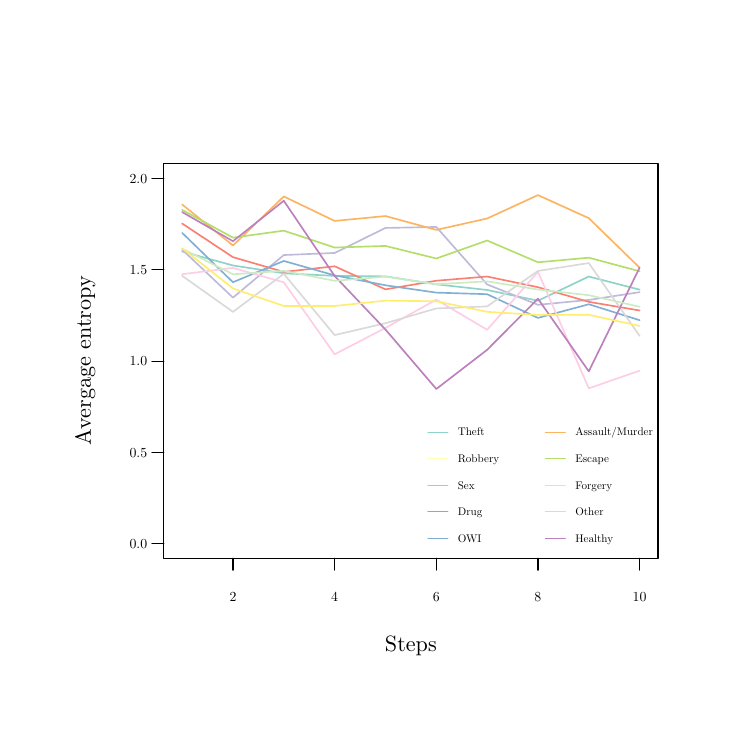
\begin{tikzpicture}[x=1pt,y=1pt]
\definecolor{fillColor}{RGB}{255,255,255}
\path[use as bounding box,fill=fillColor,fill opacity=0.00] (0,0) rectangle (252.94,252.94);
\begin{scope}
\path[clip] ( 49.20, 61.20) rectangle (227.75,203.75);
\definecolor{drawColor}{RGB}{141,211,199}

\path[draw=drawColor,line width= 0.6pt,line join=round,line cap=round] ( 55.81,172.06) --
	( 74.18,167.01) --
	( 92.55,164.18) --
	(110.92,163.25) --
	(129.29,163.07) --
	(147.66,160.20) --
	(166.03,158.15) --
	(184.39,154.27) --
	(202.76,163.01) --
	(221.13,158.27);
\end{scope}
\begin{scope}
\path[clip] (  0.00,  0.00) rectangle (252.94,252.94);
\definecolor{drawColor}{RGB}{0,0,0}

\path[draw=drawColor,line width= 0.4pt,line join=round,line cap=round] ( 74.18, 61.20) -- (221.13, 61.20);

\path[draw=drawColor,line width= 0.4pt,line join=round,line cap=round] ( 74.18, 61.20) -- ( 74.18, 56.92);

\path[draw=drawColor,line width= 0.4pt,line join=round,line cap=round] (110.92, 61.20) -- (110.92, 56.92);

\path[draw=drawColor,line width= 0.4pt,line join=round,line cap=round] (147.66, 61.20) -- (147.66, 56.92);

\path[draw=drawColor,line width= 0.4pt,line join=round,line cap=round] (184.39, 61.20) -- (184.39, 56.92);

\path[draw=drawColor,line width= 0.4pt,line join=round,line cap=round] (221.13, 61.20) -- (221.13, 56.92);

\node[text=drawColor,anchor=base,inner sep=0pt, outer sep=0pt, scale=  0.50] at ( 74.18, 45.60) {2};

\node[text=drawColor,anchor=base,inner sep=0pt, outer sep=0pt, scale=  0.50] at (110.92, 45.60) {4};

\node[text=drawColor,anchor=base,inner sep=0pt, outer sep=0pt, scale=  0.50] at (147.66, 45.60) {6};

\node[text=drawColor,anchor=base,inner sep=0pt, outer sep=0pt, scale=  0.50] at (184.39, 45.60) {8};

\node[text=drawColor,anchor=base,inner sep=0pt, outer sep=0pt, scale=  0.50] at (221.13, 45.60) {10};

\path[draw=drawColor,line width= 0.4pt,line join=round,line cap=round] ( 49.20, 66.48) -- ( 49.20,198.47);

\path[draw=drawColor,line width= 0.4pt,line join=round,line cap=round] ( 49.20, 66.48) -- ( 44.92, 66.48);

\path[draw=drawColor,line width= 0.4pt,line join=round,line cap=round] ( 49.20, 99.48) -- ( 44.92, 99.48);

\path[draw=drawColor,line width= 0.4pt,line join=round,line cap=round] ( 49.20,132.47) -- ( 44.92,132.47);

\path[draw=drawColor,line width= 0.4pt,line join=round,line cap=round] ( 49.20,165.47) -- ( 44.92,165.47);

\path[draw=drawColor,line width= 0.4pt,line join=round,line cap=round] ( 49.20,198.47) -- ( 44.92,198.47);

\node[text=drawColor,anchor=base east,inner sep=0pt, outer sep=0pt, scale=  0.50] at ( 43.20, 64.76) {0.0};

\node[text=drawColor,anchor=base east,inner sep=0pt, outer sep=0pt, scale=  0.50] at ( 43.20, 97.75) {0.5};

\node[text=drawColor,anchor=base east,inner sep=0pt, outer sep=0pt, scale=  0.50] at ( 43.20,130.75) {1.0};

\node[text=drawColor,anchor=base east,inner sep=0pt, outer sep=0pt, scale=  0.50] at ( 43.20,163.75) {1.5};

\node[text=drawColor,anchor=base east,inner sep=0pt, outer sep=0pt, scale=  0.50] at ( 43.20,196.74) {2.0};

\path[draw=drawColor,line width= 0.4pt,line join=round,line cap=round] ( 49.20, 61.20) --
	(227.75, 61.20) --
	(227.75,203.75) --
	( 49.20,203.75) --
	( 49.20, 61.20);
\end{scope}
\begin{scope}
\path[clip] (  0.00,  0.00) rectangle (252.94,252.94);
\definecolor{drawColor}{RGB}{0,0,0}

\node[text=drawColor,anchor=base,inner sep=0pt, outer sep=0pt, scale=  0.80] at (138.47, 27.60) {Steps};

\node[text=drawColor,rotate= 90.00,anchor=base,inner sep=0pt, outer sep=0pt, scale=  0.80] at ( 22.80,132.47) {Avergage entropy};
\end{scope}
\begin{scope}
\path[clip] ( 49.20, 61.20) rectangle (227.75,203.75);
\definecolor{drawColor}{RGB}{190,186,218}

\path[draw=drawColor,line width= 0.6pt,line join=round,line cap=round] ( 55.81,172.75) --
	( 74.18,155.39) --
	( 92.55,170.78) --
	(110.92,171.53) --
	(129.29,180.57) --
	(147.66,180.92) --
	(166.03,160.16) --
	(184.39,152.80) --
	(202.76,154.55) --
	(221.13,157.37);
\definecolor{drawColor}{RGB}{251,128,114}

\path[draw=drawColor,line width= 0.6pt,line join=round,line cap=round] ( 55.81,182.17) --
	( 74.18,170.01) --
	( 92.55,164.69) --
	(110.92,166.72) --
	(129.29,158.38) --
	(147.66,161.50) --
	(166.03,163.01) --
	(184.39,159.16) --
	(202.76,153.87) --
	(221.13,150.74);
\definecolor{drawColor}{RGB}{128,177,211}

\path[draw=drawColor,line width= 0.6pt,line join=round,line cap=round] ( 55.81,178.80) --
	( 74.18,160.95) --
	( 92.55,168.64) --
	(110.92,163.44) --
	(129.29,159.85) --
	(147.66,157.20) --
	(166.03,156.63) --
	(184.39,148.06) --
	(202.76,152.99) --
	(221.13,147.23);
\definecolor{drawColor}{RGB}{253,180,98}

\path[draw=drawColor,line width= 0.6pt,line join=round,line cap=round] ( 55.81,189.06) --
	( 74.18,174.23) --
	( 92.55,191.95) --
	(110.92,183.10) --
	(129.29,184.87) --
	(147.66,179.86) --
	(166.03,183.99) --
	(184.39,192.44) --
	(202.76,184.10) --
	(221.13,166.20);
\definecolor{drawColor}{RGB}{179,222,105}

\path[draw=drawColor,line width= 0.6pt,line join=round,line cap=round] ( 55.81,187.11) --
	( 74.18,177.06) --
	( 92.55,179.59) --
	(110.92,173.49) --
	(129.29,174.07) --
	(147.66,169.53) --
	(166.03,176.03) --
	(184.39,168.16) --
	(202.76,169.82) --
	(221.13,164.91);
\definecolor{drawColor}{RGB}{252,205,229}

\path[draw=drawColor,line width= 0.6pt,line join=round,line cap=round] ( 55.81,163.85) --
	( 74.18,166.13) --
	( 92.55,160.92) --
	(110.92,134.90) --
	(129.29,144.45) --
	(147.66,154.65) --
	(166.03,143.78) --
	(184.39,164.72) --
	(202.76,122.61) --
	(221.13,129.00);
\definecolor{drawColor}{gray}{0.85}

\path[draw=drawColor,line width= 0.6pt,line join=round,line cap=round] ( 55.81,163.28) --
	( 74.18,150.25) --
	( 92.55,163.99) --
	(110.92,141.86) --
	(129.29,146.14) --
	(147.66,151.49) --
	(166.03,152.22) --
	(184.39,165.03) --
	(202.76,167.88) --
	(221.13,141.56);
\definecolor{drawColor}{RGB}{188,128,189}

\path[draw=drawColor,line width= 0.6pt,line join=round,line cap=round] ( 55.81,186.32) --
	( 74.18,175.78) --
	( 92.55,190.39) --
	(110.92,163.22) --
	(129.29,143.86) --
	(147.66,122.38) --
	(166.03,136.54) --
	(184.39,155.01) --
	(202.76,128.75) --
	(221.13,166.25);
\definecolor{drawColor}{RGB}{204,235,197}

\path[draw=drawColor,line width= 0.6pt,line join=round,line cap=round] ( 55.81,173.08) --
	( 74.18,163.82) --
	( 92.55,165.07) --
	(110.92,161.47) --
	(129.29,162.96) --
	(147.66,160.23) --
	(166.03,161.27) --
	(184.39,158.32) --
	(202.76,156.27) --
	(221.13,152.10);
\definecolor{drawColor}{RGB}{255,237,111}

\path[draw=drawColor,line width= 0.6pt,line join=round,line cap=round] ( 55.81,173.25) --
	( 74.18,158.72) --
	( 92.55,152.37) --
	(110.92,152.37) --
	(129.29,154.31) --
	(147.66,154.07) --
	(166.03,150.25) --
	(184.39,149.14) --
	(202.76,149.19) --
	(221.13,145.17);
\definecolor{drawColor}{RGB}{141,211,199}

\path[draw=drawColor,line width= 0.4pt,line join=round,line cap=round] (144.63,106.80) -- (151.83,106.80);
\definecolor{drawColor}{RGB}{255,255,179}

\path[draw=drawColor,line width= 0.4pt,line join=round,line cap=round] (144.63, 97.20) -- (151.83, 97.20);
\definecolor{drawColor}{RGB}{190,186,218}

\path[draw=drawColor,line width= 0.4pt,line join=round,line cap=round] (144.63, 87.60) -- (151.83, 87.60);
\definecolor{drawColor}{RGB}{251,128,114}

\path[draw=drawColor,line width= 0.4pt,line join=round,line cap=round] (144.63, 78.00) -- (151.83, 78.00);
\definecolor{drawColor}{RGB}{128,177,211}

\path[draw=drawColor,line width= 0.4pt,line join=round,line cap=round] (144.63, 68.40) -- (151.83, 68.40);
\definecolor{drawColor}{RGB}{253,180,98}

\path[draw=drawColor,line width= 0.4pt,line join=round,line cap=round] (187.09,106.80) -- (194.29,106.80);
\definecolor{drawColor}{RGB}{179,222,105}

\path[draw=drawColor,line width= 0.4pt,line join=round,line cap=round] (187.09, 97.20) -- (194.29, 97.20);
\definecolor{drawColor}{RGB}{252,205,229}

\path[draw=drawColor,line width= 0.4pt,line join=round,line cap=round] (187.09, 87.60) -- (194.29, 87.60);
\definecolor{drawColor}{gray}{0.85}

\path[draw=drawColor,line width= 0.4pt,line join=round,line cap=round] (187.09, 78.00) -- (194.29, 78.00);
\definecolor{drawColor}{RGB}{188,128,189}

\path[draw=drawColor,line width= 0.4pt,line join=round,line cap=round] (187.09, 68.40) -- (194.29, 68.40);
\definecolor{drawColor}{RGB}{0,0,0}

\node[text=drawColor,anchor=base west,inner sep=0pt, outer sep=0pt, scale=  0.40] at (155.43,105.42) {Theft};

\node[text=drawColor,anchor=base west,inner sep=0pt, outer sep=0pt, scale=  0.40] at (155.43, 95.82) {Robbery};

\node[text=drawColor,anchor=base west,inner sep=0pt, outer sep=0pt, scale=  0.40] at (155.43, 86.22) {Sex};

\node[text=drawColor,anchor=base west,inner sep=0pt, outer sep=0pt, scale=  0.40] at (155.43, 76.62) {Drug};

\node[text=drawColor,anchor=base west,inner sep=0pt, outer sep=0pt, scale=  0.40] at (155.43, 67.02) {OWI};

\node[text=drawColor,anchor=base west,inner sep=0pt, outer sep=0pt, scale=  0.40] at (197.89,105.42) {Assault/Murder};

\node[text=drawColor,anchor=base west,inner sep=0pt, outer sep=0pt, scale=  0.40] at (197.89, 95.82) {Escape};

\node[text=drawColor,anchor=base west,inner sep=0pt, outer sep=0pt, scale=  0.40] at (197.89, 86.22) {Forgery};

\node[text=drawColor,anchor=base west,inner sep=0pt, outer sep=0pt, scale=  0.40] at (197.89, 76.62) {Other};

\node[text=drawColor,anchor=base west,inner sep=0pt, outer sep=0pt, scale=  0.40] at (197.89, 67.02) {Healthy};
\end{scope}
\end{tikzpicture}
